\documentclass[12pt,a4paper]{article}
\usepackage{cmap} % Makes the PDF copiable. See http://tex.stackexchange.com/a/64198/25761
\usepackage[T1]{fontenc}
\usepackage[brazil]{babel}
\usepackage[utf8]{inputenc}
\usepackage{amsmath}
\usepackage{amsfonts}
\usepackage{amssymb}
\usepackage{amsthm}
\usepackage{textcomp} % \degree
\usepackage{gensymb} % \degree
\usepackage[usenames,svgnames,dvipsnames]{xcolor}
\usepackage{hyperref}
\usepackage{multicol}
\usepackage{graphicx}
\usepackage[margin=2cm]{geometry}
\usepackage{systeme}

\hypersetup{
    colorlinks = true,
    allcolors = {blue}
}

% TODO: Consider using exsheets
% http://linorg.usp.br/CTAN/macros/latex/contrib/exsheets/exsheets_en.pdf
%
% http://ctan.org/tex-archive/macros/latex/contrib/exercise/
% Options: answerdelayed,lastexercise,noanswer
\usepackage[answerdelayed,lastexercise]{exercise}

\addto\captionsbrazil{%
\def\listexercisename{Lista de exerc\'icios}%
\def\ExerciseName{Exerc\'icio}%
\def\AnswerName{Solu\c{c}\~ao do exerc\'icio}%
\def\ExerciseListName{Ex.}%
\def\AnswerListName{Solu\c{c}\~ao}%
\def\ExePartName{Parte}%
\def\ArticleOf{de\ }%
}

\renewcommand{\ExerciseHeaderTitle}{(\ExerciseTitle)\ }
\renewcommand{\ExerciseListHeader}{%\ExerciseHeaderDifficulty%
\textbf{%\ExerciseListName\
\ExerciseHeaderNB.\ %
%\ --- \
\ExerciseHeaderTitle}%
%\ExerciseHeaderOrigin
\ignorespaces}
\renewcommand{\AnswerListHeader}{\textbf{\ExerciseHeaderNB.\ (\AnswerListName)\ }}

\newcommand*\R{\mathbb{R}}

% Loop Space / CC BY-SA-3.0 / https://tex.stackexchange.com/a/2238/25761
\newenvironment{amatrix}[1]{%
  \left[\begin{array}{@{}*{#1}{c}|c@{}}
}{%
  \end{array}\right]
}

% Loop Space / CC BY-SA-3.0 / https://tex.stackexchange.com/a/3164/25761
%--------grstep
% For denoting a Gauss' reduction step.
% Use as: \grstep{\rho_1+\rho_3} or \grstep[2\rho_5 \\ 3\rho_6]{\rho_1+\rho_3}
\newcommand{\grstep}[2][\relax]{%
   \ensuremath{\mathrel{
       {\mathop{\longrightarrow}\limits^{#2\mathstrut}_{
                                     \begin{subarray}{l} #1 \end{subarray}}}}}}

\renewcommand{\theenumi}{\alph{enumi}}
\renewcommand\labelenumi{(\theenumi) }

\newcommand*\tipo{Prova I}
\newcommand*\turma{PRO112-02U}
\newcommand*\disciplina{ALI0001}
\newcommand*\eu{Helder G. G. de Lima}
\newcommand*\data{04/09/2017}

\author{\eu}
\title{\tipo - \disciplina}
\date{\data}

\begin{document}
\thispagestyle{empty}
\newgeometry{margin=2cm,bottom=0.5cm}
\begin{center}

\includegraphics[width=9.0cm]{marca} \\
\textbf{\tipo\ (\disciplina / \turma)} \\
Prof. \eu\footnote{
Este é um material de acesso livre distribuído sob os termos da licença \href{https://creativecommons.org/licenses/by-sa/4.0/deed.pt_BR}{Creative Commons BY-SA 4.0}}
\end{center}

\noindent Nome do(a) aluno(a): \underline{\hspace{9,7cm}} Data: \underline{\data}

%\section*{Instruções}
\begin{center}\fbox{
\begin{minipage}{14cm}

{\footnotesize
\begin{itemize}
\renewcommand{\theenumi}{\Roman{enumi}}
\item Identifique-se em todas as folhas.
\item Mantenha o celular e os demais equipamentos eletrônicos desligados durante a prova.
\item Resolva (integralmente) apenas os itens de que precisar para somar 10,0 pontos.
\end{itemize}
}

\end{minipage}
}
\end{center}

\section*{Questões}
\begin{ExerciseList}
\Exercise[title={2,5}]
Encontre todos os valores de $a$ e $b$ para os quais o sistema linear \systeme[xy]{
-x + 3y = 5,
 x - ay = b
}
é possível e determinado. Há alguma escolha de $a$ e $b$ que resulta em um sistema impossível? Em que caso(s) existirão infinitas soluções para este sistema?
\Answer Se $a \neq 3$, esta é a forma escalonada reduzida da matriz ampliada do sistema:
\[
\begin{bmatrix}
-1 & 3 & 5 \\
 1 & -a & b
\end{bmatrix}
\rightarrow
\begin{bmatrix}
-1 & 3 & 5 \\
 0 & -a+3 & b+5
\end{bmatrix}
\rightarrow
\begin{bmatrix}
1 & -3 & -5 \\
0 &  1 & \frac{b+5}{-a+3}
\end{bmatrix}
\rightarrow
\begin{bmatrix}
1 & 0 & \frac{5a+3b}{-a+3} \\
0 & 1 & \frac{b+5}{-a+3}
\end{bmatrix}
\]
Então o sistema é possível e determinado para todo $a \neq 3$. Por outro lado, se $a = 3$, o posto da matriz (não ampliada) do sistema é $1$, e ele pode ser classificado como:
\begin{enumerate}
\item Impossível, se $b \neq -5$ (pois o posto da matriz ampliada será $2 > 1$).
\item Possível e indeterminado, se $b = -5$ (pois o posto da matriz ampliada também será $1$).
\end{enumerate}


\Exercise[title={2,5}]
\begin{minipage}[t]{0.6\textwidth}
O volume de carros que circulam por hora nos entornos da praça central de uma cidade é mostrado ao lado.
\begin{enumerate}
\item Com as informações dadas, é possível saber qual é o volume de tráfego nos trechos $x_1, \ldots, x_4$?
\item Nas condições dadas, seria possível que $x_4 = 0$ (por exemplo, devido a uma interdição naquela rua)? Justifique suas respostas.
\end{enumerate}
\end{minipage}
\hfill
\begin{minipage}[t]{0.3\textwidth}
\raggedleft
\vfill
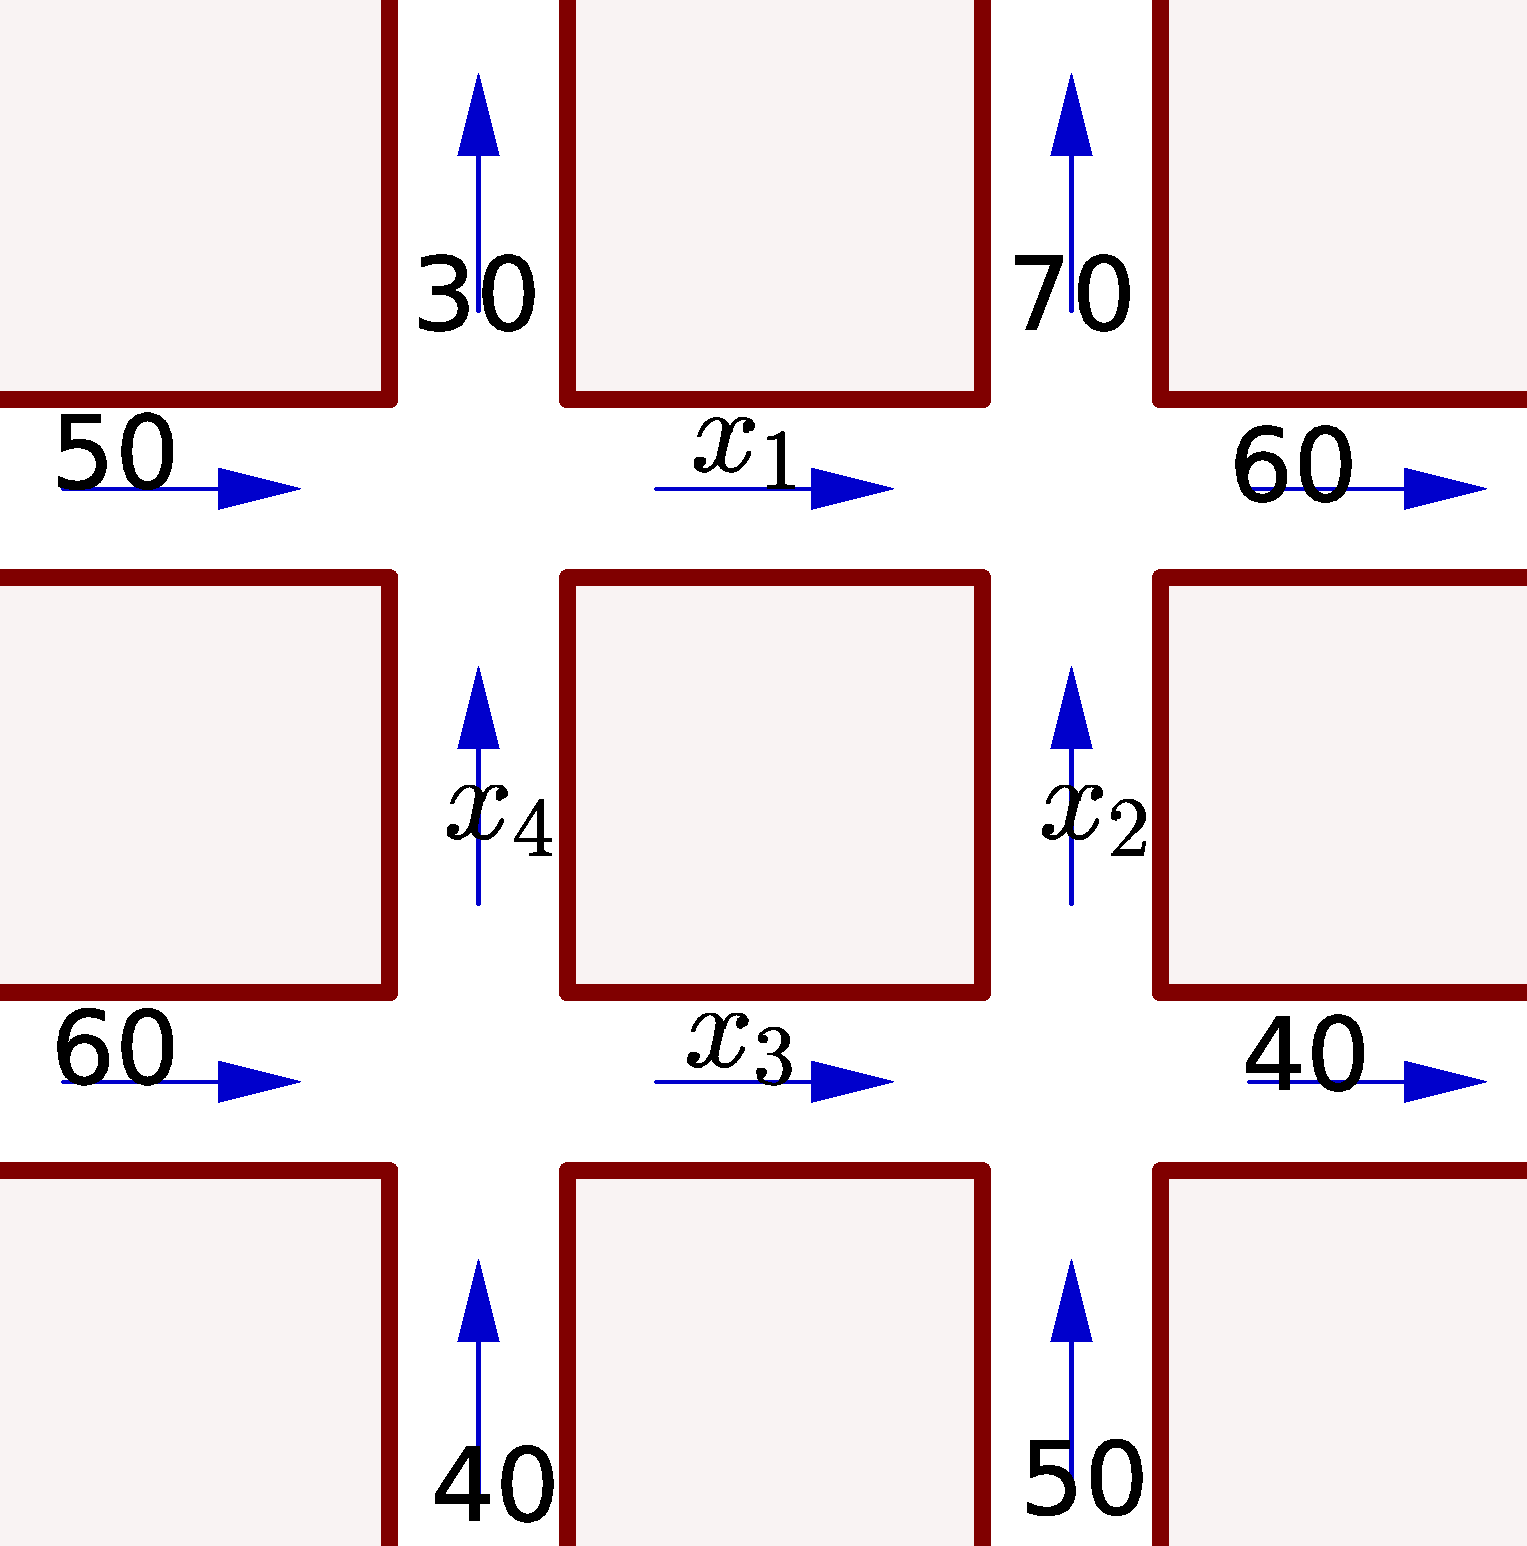
\includegraphics[width=4.6cm]{img/prova-1-pro-quadras}
\end{minipage}
\Answer O número de carros que entram em cada cruzamento deve ser igual ao de carros que saem, então $x_1, \ldots, x_4$ devem satisfazer estas equações:

$\begin{cases}
x_1 + x_2 & = 70 + 60\\
x_3 +  50 & = x_2 + 40\\
60 + 40   & = x_3 + x_4\\
50 + x_4    & = 30 + x_1,
\end{cases}$
que equivalem a
\systeme[x_1x_2x_3x_4]{
 x_1 + x_2 = 130,
-x_2 + x_3 = -10,
 x_3 + x_4 = 100,
-x_1 + x_4 = -20
}

Procedendo com o escalonamento do sistema, obtém-se:
{\footnotesize
\begin{align*}
\begin{bmatrix}
 1 &  1 & 0 & 0 & 130 \\
 0 & -1 & 1 & 0 & -10 \\
 0 &  0 & 1 & 1 & 100 \\
-1 &  0 & 0 & 1 & -20
\end{bmatrix}
\rightarrow
& \begin{bmatrix}
 1 &  1 & 0 & 0 & 130 \\
 0 & -1 & 1 & 0 & -10 \\
 0 &  0 & 1 & 1 & 100 \\
 0 &  1 & 0 & 1 & 110
\end{bmatrix}
\rightarrow
\begin{bmatrix}
 1 &  1 &  0 & 0 & 130 \\
 0 &  1 & -1 & 0 &  10 \\
 0 &  0 &  1 & 1 & 100 \\
 0 &  1 &  0 & 1 & 110
\end{bmatrix}
\rightarrow
\begin{bmatrix}
 1 &  1 &  0 & 0 & 130 \\
 0 &  1 & -1 & 0 &  10 \\
 0 &  0 &  1 & 1 & 100 \\
 0 &  0 &  1 & 1 & 100
\end{bmatrix} \\
\rightarrow
&\begin{bmatrix}
 1 &  1 &  0 & 0 & 130 \\
 0 &  1 & -1 & 0 &  10 \\
 0 &  0 &  1 & 1 & 100 \\
 0 &  0 &  0 & 0 &   0
\end{bmatrix}
\rightarrow
\begin{bmatrix}
 1 &  1 &  0 & 0 & 130 \\
 0 &  1 &  0 & 1 & 110 \\
 0 &  0 &  1 & 1 & 100 \\
 0 &  0 &  0 & 0 &   0
\end{bmatrix}
\rightarrow
\begin{bmatrix}
 1 &  0 &  0 & -1 & 20 \\
 0 &  1 &  0 &  1 & 110 \\
 0 &  0 &  1 &  1 & 100 \\
 0 &  0 &  0 &  0 &   0
\end{bmatrix}
\end{align*}
}
Portanto, o sistema é possível e indeterminado, com
$x_1 =  20 + x_4$,
$x_2 = 110 - x_4$ e
$x_3 = 100 - x_4$, e não é possível saber o volume de tráfego nos trechos indicados. No entanto, é perfeitamente possível que $x_4 = 0$, pois nesse caso resultaria que $x_1 = 20$, $x_2 = 110$ e $x_3 = 100$.

\Exercise[title={2,5}]
Prove (não exemplifique) se for verdadeiro, e dê um contraexemplo se for falso:
\begin{enumerate}
\item Se $A \in \R^{n \times n}$ é uma matriz diagonal, cujas entradas na diagonal são todas iguais, então $AB = BA$, qualquer que seja $B \in \R^{n \times n}$.
\item Sempre que duas matrizes $A$ e $B$ são inversíveis, também ocorre que $A^{-1} + B^{-1}$ é inversível.
\end{enumerate}
\Answer
\begin{enumerate}
\item \textbf{Verdadeiro}. Se as entradas da diagonal de $A$ são todas iguais a $k$ então $A$ é um múltiplo da matriz identidade, isto é, $A = k I$. Logo, para toda $B \in \R^{n \times n}$, tem-se:
\[
A B = (k I) B = k (I B) = k B = k (B I) = B (k I) = B A.
\]
\textbf{Alternativa 2:} pode-se calcular explicitamente as entradas de $AB$ e $BA$, que serão iguais:
\begin{align*}
[AB]_{ij}
& = a_{i1}b_{1j} + \ldots + a_{ii}b_{ij} + \ldots + a_{in}b_{nj}\\
& = 0 b_{1j} + \ldots + 0 b_{i,j-1} + k b_{ij} + 0b_{i,j+1} + \ldots + 0 b_{nj} = k b_{ij},\\
[BA]_{ij}
& = b_{i1}a_{1j} + \ldots + b_{ii}a_{ij} + \ldots + b_{in}a_{nj}\\
& = b_{1j}0 + \ldots + b_{i,j-1} 0 + b_{ij} k + b_{i,j+1}0 + \ldots + b_{nj}0 = b_{ij} k = k b_{ij}.
\end{align*}

\item \textbf{Falso}. Por exemplo, as matrizes $A = \begin{bmatrix}3\end{bmatrix}\in \R^{1 \times 1}$ e
$B = \begin{bmatrix}-3\end{bmatrix}\in \R^{1 \times 1}$ são inversíveis. Porém,
\[
  A^{-1} + B^{-1}
= \begin{bmatrix}1/3\end{bmatrix}
+ \begin{bmatrix}-1/3\end{bmatrix}
= \begin{bmatrix}0\end{bmatrix},
\]
que não é uma matriz inversível. Na verdade, dada qualquer matriz inversível $A$ de ordem $n \times n$, a matriz $B = -A$ também é inversível e
\[
  A^{-1} + B^{-1}
= A^{-1} + (-A)^{-1}
= A^{-1} - A^{-1}
= 0,
\]
que não é inversível.
\end{enumerate}

\Exercise[title={2,5}] Suponha que $A$, $B$ e $X$ sejam matrizes quadradas tais que $(2X + B)^T \cdot A = (B \cdot X)^T$.
\begin{enumerate}
\item Mostre que se $(2A^T - B)$ for inversível então $X = -(2A^T - B)^{-1} \cdot A^T \cdot B$
\item Calcule $X$, se for possível, no caso em que $A =
\begin{bmatrix}
1 & -1 & 1 \\
0 &  0 & 0 \\
0 &  0 & 0
\end{bmatrix}$ e $B =
\begin{bmatrix}
  2 & -5 &  4 \\
 -2 &  1 & -1 \\
5/3 &  0 &  0
\end{bmatrix}
$.
\end{enumerate}
\Answer
\begin{enumerate}
\item Considerando as propriedades das operações matriciais, tem-se:
\begin{align*}
  (2X + B)^T \cdot A = (B \cdot X)^T
& \Leftrightarrow
  A^T \cdot (2X + B) = B \cdot X \\
& \Leftrightarrow
  A^T \cdot (2X) + A^T \cdot B = B \cdot X \\
& \Leftrightarrow
  2 A^T \cdot X - B \cdot X = -A^T \cdot B \\
& \Leftrightarrow
  (2 A^T - B) \cdot X = -A^T \cdot B \\
& \Leftrightarrow
  X = (2 A^T - B)^{-1} \cdot (-A^T \cdot B) \\
& \Leftrightarrow
  X = - (2 A^T - B)^{-1} \cdot A^T \cdot B.
\end{align*}
\item Considerando as matrizes dadas, e o resultado anterior, tem-se:
\[
2A^T - B =
\begin{bmatrix}
 2 & 0 & 0 \\
-2 & 0 & 0 \\
 2 & 0 & 0
\end{bmatrix}
-
\begin{bmatrix}
  2 & -5 &  4 \\
 -2 &  1 & -1 \\
5/3 &  0 &  0
\end{bmatrix}
=
\begin{bmatrix}
  0 &  5 & -4 \\
  0 & -1 &  1 \\
1/3 &  0 &  0
\end{bmatrix}.
\]
A inversa dessa matriz pode ser obtida assim:
\begin{align*}
\begin{bmatrix}
  0 &  5 & -4 & 1 & 0 & 0 \\
  0 & -1 &  1 & 0 & 1 & 0 \\
1/3 &  0 &  0 & 0 & 0 & 1
\end{bmatrix}
\rightarrow
& \begin{bmatrix}
1/3 &  0 &  0 & 0 & 0 & 1 \\
  0 & -1 &  1 & 0 & 1 & 0 \\
  0 &  5 & -4 & 1 & 0 & 0
\end{bmatrix}
\rightarrow
\begin{bmatrix}
1 & 0 &  0 & 0 &  0 & 3 \\
0 & 1 & -1 & 0 & -1 & 0 \\
0 & 5 & -4 & 1 &  0 & 0
\end{bmatrix} \\
\rightarrow
& \begin{bmatrix}
1 & 0 &  0 & 0 &  0 & 3 \\
0 & 1 & -1 & 0 & -1 & 0 \\
0 & 0 &  1 & 1 &  5 & 0
\end{bmatrix}
\rightarrow
\begin{bmatrix}
1 & 0 & 0 & 0 & 0 & 3 \\
0 & 1 & 0 & 1 & 4 & 0 \\
0 & 0 & 1 & 1 & 5 & 0
\end{bmatrix}.
\end{align*}

Então
\begin{align*}
X
& = - (2 A^T - B)^{-1} \cdot A^T \cdot B
= - \begin{bmatrix}
0 & 0 & 3 \\
1 & 4 & 0 \\
1 & 5 & 0
\end{bmatrix}
\cdot
\begin{bmatrix}
 1 & 0 & 0 \\
-1 & 0 & 0 \\
 1 & 0 & 0
\end{bmatrix}
\cdot B \\
& =
-
\begin{bmatrix}
 3 & 0 & 0 \\
-3 & 0 & 0 \\
-4 & 0 & 0
\end{bmatrix}
\cdot
\begin{bmatrix}
  2 & -5 &  4 \\
 -2 &  1 & -1 \\
5/3 &  0 &  0
\end{bmatrix}
=
-
\begin{bmatrix}
 6 & -15 &  12 \\
-6 &  15 & -12 \\
-8 &  20 & -16
\end{bmatrix}
=
\begin{bmatrix}
-6 &  15 & -12 \\
 6 & -15 &  12 \\
 8 & -20 &  16
\end{bmatrix}.
\end{align*}
\end{enumerate}

\Exercise[title={2,5}] Calcule $\det{(2 (M^{-1}))}$, considerando que
$M = \begin{bmatrix}
0 & 0 & 0 &  2 & 0\\
1 & 6 & 1 & -3 & 0\\
1 & 0 & 2 &  5 & 3\\
3 & 0 & 2 &  8 & 1\\
1 & 4 & 1 &  4 & 0
\end{bmatrix}$.
\Answer Observando que
$\det{(2 (M^{-1}))}
= 2^5 \det{(M^{-1})}
= 32 \det{(M^{-1})}$,
basta calcular $\det{(M)}$. Utilizando a expansão em cofatores, obtém-se:
\begin{align*}
\det{(M)}
&= 2(-1)^{1+4}\begin{vmatrix}
1 & \textbf{6} & 1 & 0\\
1 & \textbf{0} & 2 & 3\\
3 & \textbf{0} & 2 & 1\\
1 & \textbf{4} & 1 & 0
\end{vmatrix}
= (-2)
\left(
6(-1)^{1+2}
\begin{vmatrix}
1 & 2 & 3\\
3 & 2 & 1\\
1 & 1 & 0
\end{vmatrix}
+ 4(-1)^{4+2}
\begin{vmatrix}
1 & 1 & 0\\
1 & 2 & 3\\
3 & 2 & 1\\
\end{vmatrix}
\right) \\
&=(-2)
\left(
(-6) \times 4
+ 4 \times 4
\right)
= 16.
\end{align*}
Logo, $\det{(2 (M^{-1}))} = \frac{ 32 }{ 16 } = 2$.

\textbf{Alternativa 2}: Poderiam ser usadas operações elementares para triangularizar a matriz $M$.
\textbf{Alternativa 3}: Poderia ser calculada a inversa explicitamente, e só então calcular o seu determinante, mas essa é uma opção muito menos eficiente.
\end{ExerciseList}

\begin{center}
BOA PROVA!
\end{center}

\newpage
\restoregeometry
\section*{Respostas}
\shipoutAnswer
\end{document}
